\chapter{Introduction and Scope}

\epigraph{\emph This chapter provides background information on education system and learning methods. It then sheds some light into education system in Cambodia, and highlights the needs to enable technology-based education. Finally, it presents the objectives and methodology of this practicum.}{}

\newpage




\section{Background}


As Nelson Mandela famously said, “Education is the most powerful weapon which you can use to change the world.” It is an essential part of our lives and it builds the platform for development of all kinds of necessary skills. Of many ways a person can be educated, such as by experiences, schooling, training, and research among others, teaching through direct guidance has always been the most common and formal method. The techniques of teaching have evolved from traditional blackboard-chalk to slides and overhead projectors to the use of softwares and then to videos, and network resources \citep{DELCAMPO2012TRA}.


At the same time, learning in different environment has also changed from being fixed to fluid, as one can learn things in a multi-dimensional way through multiple media. And, there is increased recognition that one medium of teaching is insufficient \citep{ref701470815} (available for download\footnote{\url{http://sites.duke.edu/arthist110_001_f2011/files/2011/08/Thomas_Brown_A_New_Culture_of_Learning.pdf}}). Therefore, technology is being used in the classroom not just in computer-related courses, but also in other courses like English, Maths and Science as well.  


In many cases, it has been suggested that difference in learning styles has lead to difference in achievements, as educational systems have not adapted to the changes in technology and there is a need to better regulate learning through effective learning techniques \citep{dunlosky2013improving}.


But, in general, the pedagogical issues of technology-based education have been raised in the developed countries, where technology has been used in education for much longer than a decade. In the wider perspective of whole world, the situation is even grimmer. According to UNESCO\footnote{\url{http://www.un.org/en/globalissues/children/pdf/educationfirst-facts.pdf}}, 61 million primary school-age children did not have access to school in 2010. But, even for those going to schools, the resources are limited and traditional methods are exclusively used for teaching. 

Due to poor quality of education in many developing countries, even children with primary level education may lack basic skills\footnote{\url{http://www.bmz.de/en/what\_we\_do/issues/Education/hintergrund/bildungsituation/}}. The overloaded courses often lack clear targets, do not meet the learning needs, and ignore social, cultural and regional factors. As such, the education is not in line with the everyday lives of children, which inhibits learning. 

But over the last decade, it has been shown that with proper resources in developing countries, technology-enabled learning are more effective for both teachers and students \citep{Bransford00whencomputer,fisher2010technology}, and significant increase in academic achievements have been reported. For example, One Laptop per Child\footnote{\url{http://one.laptop.org}}, which provides \$100 laptops for children, 
and Hole-in-The-Wall Education Limited\footnote{\url{http://www.hole-in-the-wall.com}}, which provides access to computing facility in rural areas, report improvement in collaborative learning abilities and engaging activities of the children. 

With a near exponential increase in availability of affordable technology across the world, there is a new and exciting opportunity to improve the education in the most impoverished countries through the use of technology.

\section{Context and Need}

As discussed in previous section, the education system in developing countries are often limited by both resources and methods. Group work, independent learning, critical thought and problem solving, the use of new technologies and the development of life skills are, often, neglected. 

The target beneficiaries of the findings of this practicum are school children in rural Cambodia. This practicum was carried out in collaboration with Children's Future Organization (CFO)\footnote{\url{http://www.childrensfuture.org}}, a Denver-based International Non-Governmental Organization, which has been working in Cambodia since 2008. Their primary mission is to help break the cycle of poverty by providing the country’s poorest and most vulnerable children an opportunity to become educated, self-reliant and compassionate individuals.
With that in mind, CFO opened a Learning Center in rural Cambodia in 2010. The Learning Center is the nucleus for all of CFO's work in the area. More than 230 children are enrolled and they are supported by diligent work of dedicated staff and volunteers, which includes teachers, social workers and housemothers.

In Cambodia, the traditional education was gradually replaced during the time as a part of French colony\footnote{\url{http://www.bookbridge.org/2012/03/the-education-system-in-cambodia/}}. A western education model was introduced in a formal education system then. But, following years of civil wars, the education system was strongly affected and was completely destroyed during the Red Khmer regime (1970s). Between 1980s and 1990s, the efforts to rebuild education system from scratch were initialized and it has gradually developed since.


The general education is now based on a national school curriculum that is classified into basic and upper secondary education. The basic education consists of three cycles of three years each. The first, second, and third cycle consist of 27-30, 30-32, and 32-35 40-minutes long lessons per week, respectively. All three cycles of basic education have the following subject matters\footnote{\url{http://www.ibe.unesco.org/fileadmin/user_upload/archive/Countries/WDE/2006/ASIA_and_the_PACIFIC/Cambodia/Cambodia.htm}}.
\begin{itemize}
 \item Khmer language and literature
\item        Mathematics
\item         Sciences (Physics, Chemistry, Biology, and Earth \& Environmental Studies)
\item          Social Studies (History, Geography, economics, Art, and Morals and Civics)
\item     Foreign Languages
\item          Health and Physical Education and Sport

\end{itemize}

Almost half of the lessons are for the national language Khmer spoken by 13 million people. The local life skills lessons are included in all three cycles but they are mostly focused on literature, the foundation of religion, and skills for daily life like carpentry, artistry, craftwork, constructing, playing instruments etc. More importantly, there are no courses related to information and communication technology (ICT) during the first 10 school years, and it is only offered as an option in 11-12$\mathrm{^{th}}$ year of school education. As children have larger cognitive skills, the missing life skills related to ICT seriously hinders the ability of students, and the usefulness of education in careers requiring such expertise.

In terms of learning skills, education systems without ICT are less effective in implementing a flexible method. Previous research has shown that provided the resources, there is evidence that technology can, and does, support learning and promotes communication skills \citep{marshall2002}. Similarly, the flexibility is an important aspect, as there can be a clear difference in teaching, learning and application based on individual differences \citep{Ayersman1995371}. In fact, UNESCO has highlighted the need for a personalized curriculum and a critical role of ICT by suggesting that “one size fits all" education system does not allow students to achieve their best possible learning results\footnote{\url{http://iite.unesco.org/publications/3214716/}}. Other studies have also shown that there can be a significant increase in academic achievement with use of technology \citep{zywno2002effect}. 

Thus, there is a clear need of enabling ICT supported education system in Cambodia for the following reasons:
\begin{itemize}
	\item To improve the cognitive skills of children in school education.
	\item To provide flexible system to improve the learning and make sure that each student reaches the maximum potential.
	\item To elevate the level of academic achievement.
\end{itemize}

\section{Objectives}

The overall aim of this practicum is to evaluate the commonly-used and available resources that can support the use of technological advances in improving the education system in a school, the Learning Center of CFO, in rural Cambodia. More specifically, the objectives can be listed as,

\begin{enumerate}
\item Evaluate the resources available for using technology such as computers, mobile devices, etc. in primary school education.
\item Identify a tool to improve the learning environment for children and provide hands on information and tutorials to use the tool.
\item Create a platform to share the knowledge and experiences. 

\end{enumerate}

\section{Methodology}

This practicum has four basic aspects; explore, design, display and distribute. A simple mind map of the scope is presented in Figure~\ref{fig:workflow}. “Explore" represents the aspect of the work that is focused on exploring the education methods and providing hands-on review of the currently available resources (discussed in Chapter 2). “Design" focuses on how an effective course can be designed based on learning methods dependent on technology (Chapter 3). “Display" focuses on creation of example courses for some subject matters (Chapter 3 and website). “Distribute" represents the development of a web-based platform to share the knowledge and experiences.

\usetikzlibrary{mindmap,trees}


\begin{figure}[h!]
\tikzset{every node/.append style={scale=0.95}}
%\tikzset{every node/.append style={scale=0.9, minimum size=3.6cm}}

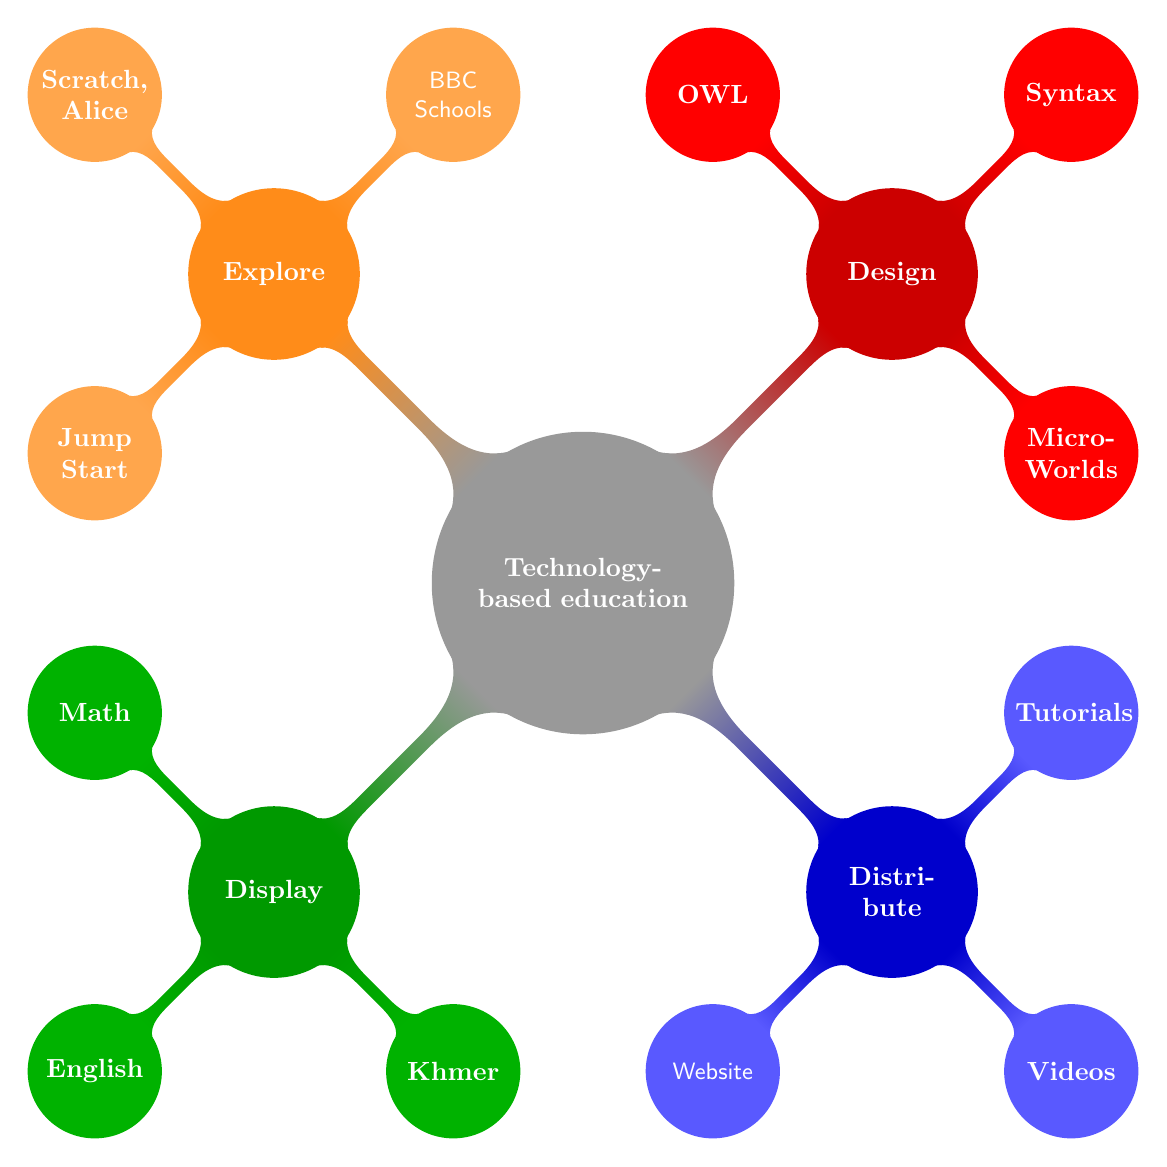
\begin{tikzpicture}[mindmap, concept color=gray!80, font=\sf, text=white,scale=1.11]
\centering

  \tikzstyle{level 1 concept}+=[font=\sf\bf, sibling angle=90]
  \tikzstyle{level 2 concept}+=[font=\sf\bf, sibling angle=90]
 
  \node[concept]{\bf Technology-based education}[clockwise from=45]
    child[concept color=red!80!black, grow=right,clockwise from=45]
    {
        node[concept]{Design}[clockwise from=135]
            child[concept color=red]{ node[concept]{OWL}}
            child[concept color=red]{ node[concept]{Syntax}}
            child[concept color=red]{ node[concept]{Micro-  Worlds}}
    }
    child[concept color=blue!80!black]
    {
        node[concept]{Distri- bute}[clockwise from=45]
            child[concept color=blue!65]{ node[concept]{Tutorials}}
            child[concept color=blue!65]{ node[concept]{Videos}}
            child[concept color=blue!65, font=\sf \small]{ node[concept]{Website}}
    }
    child[concept color=green!60!black]
    {
        node[concept]{Display}[clockwise from=315]
            child[concept color=green!70!black]{ node[concept]{Khmer}}
            child[concept color=green!70!black]{ node[concept]{English}}
            child[concept color=green!70!black]{ node[concept]{Math}}
    }
    child[concept color=orange!90]
    { 
        node[concept]{Explore}[clockwise from=225]
            child[concept color=orange!70]{ node[concept]{Jump Start}}
            child[concept color=orange!70]{ node[concept]{Scratch, Alice}}
            child[concept color=orange!70, font=\sf \small]{ node[concept]{BBC Schools}}
    };

\end{tikzpicture}
\captionsetup{justification=centering,margin=2cm}
\caption{Mind map of components of the practicum}

\label{fig:workflow}
\end{figure}
    




